%\documentstyle[epsf,twocolumn]{jarticle}       %LaTeX2e仕様
\documentclass[twocolumn]{jarticle}     %pLaTeX2e仕様(platex.exeの場合)
%\documentclass[twocolumn]{ujarticle}     %pLaTeX2e仕様(uplatex.exeの場合)
%%%%%%%%%%%%%%%%%%%%%%%%%%%%%%%%%%%%%%%%%%%%%%%%%%%%%%%%%%%%%%
%%
%%  基本バージョン
%%
%%%%%%%%%%%%%%%%%%%%%%%%%%%%%%%%%%%%%%%%%%%%%%%%%%%%%%%%%%%%%%%%
\setlength{\topmargin}{-45pt}
%\setlength{\oddsidemargin}{0cm} 
\setlength{\oddsidemargin}{-7.5mm}
%\setlength{\evensidemargin}{0cm} 
\setlength{\textheight}{24.1cm}
%setlength{\textheight}{25cm} 
\setlength{\textwidth}{17.4cm}
%\setlength{\textwidth}{172mm} 
\setlength{\columnsep}{11mm}

\kanjiskip=.07zw plus.5pt minus.5pt


% 【節が変わるごとに (1.1)(1.2) … (2.1)(2.2) と数式番号をつけるとき】
%\makeatletter
%\renewcommand{\theequation}{%
%\thesection.\arabic{equation}} %\@addtoreset{equation}{section}
%\makeatother

%\renewcommand{\arraystretch}{0.95} 行間の設定

%%%%%%%%%%%%%%%%%%%%%%%%%%%%%%%%%%%%%%%%%%%%%%%%%%%%%%%%
\usepackage[dvipdfmx]{graphicx}   %pLaTeX2e仕様(\documentstyle ->\documentclass)\documentclass[dvipdfmx]{graphicx}
\usepackage[dvipdfmx]{color}
\usepackage[subrefformat=parens]{subcaption}
\usepackage{colortbl}
%%%%%%%%%%%%%%%%%%%%%%%%%%%%%%%%%%%%%%%%%%%%%%%%%%%%%%%%

\begin{document}

\twocolumn[
\noindent

\hspace{1em}
\today
\hfill
\ \ 細川 岳大

\vspace{2mm}

\hrule

\begin{center}
{\Large \bf 進捗報告}
\end{center}
\hrule
\vspace{3mm}
]

% ‚ここから 文章 Start!
\section{今週やったこと}
 GAを用いたDataAugmentaion

\section{実験1}
前回に引き続きGAを用いたDataAugmentationの実験を行った.\\

\subsection{実験データ}
実験データはcifar10を用いて,
事前学習ではepoch数300,train\_dataを各ラベル5000枚の計50000枚使用し,GAで学習する際はepoch数100,train\_dataは各ラベル200枚のオリジナルとそれらすべてをDataAugmentaionしたものとを合わせ計4000枚とし,test\_dataは共に10000枚とした.また事前学習でのaccuracyは0.8475である.
\subsection{遺伝的アルゴリズム}


\subsubsection{探索空間}
\ 探索する水増し操作として画素値操作(Sharpness,Posterize,Brightness,Autoconstrast,Equalize,Solarize,Invert,Contrast,ColorBalance),
変形操作(Mirror,Flip,Translate X/Y,Shear X/Y,Rotate)の16種類の操作であり,今回はそれらすべてを個別にどの程度強くかけるかおよびどの順序でかけるかということを探索する.各操作についての強度の最大最小を設定し,それを-100\%から100\%まで25\%ずつ分11段階の度合いとする.ただし,Autocontrast,Equalize,Invert,Mirror については適用するか否かであるためパラメータが0以上で適用するとした.強度は0から5の整数値を持つ15個の遺伝子を実数値コーディングによって表現する.
また,適用順序に関しては同様に15個の遺伝子を持つ順列コーディングによって表現する.
確率は10\%ごと11段階の実数地コーディングによって表現する.
つまり,探索空間は$2^5*11^{11}*15!*11^{16}$となる.

\subsubsection{選択}
\ 選択について,エリート選出によって最も適応度の高い2つの個体を選択する.なお,この二つは後述する交叉,突然変異は受けずに次の世代に追加する.
残りの選出にはトーナメント選出を用した.トーナメント選出は集団の中から任意の数(トーナメントサイズ)の個体のうち最も適応度の高い個体を選出し次の世代に追加する.今回トーナメントサイズは2とした.
 
\subsubsection{交叉}
\ 強度,確率を表す染色体については2点交叉,順序を表す染色体については部分写像交叉を用いた.2点交叉は一対の親染色体をそれぞれ同じ場所で三分割し中央の染色体を入れ替えて交叉を行う.部分写像交叉は親遺伝子を二分割し入れ替える際重複をなくす交叉法で,重複のあった遺伝子について,それに該当した重複する遺伝子座を見つけ,それに対となっているもう一方の親の遺伝子を参照する.
 
\subsubsection{突然変異}
\ 強度,確率を表す染色体について,対象となる遺伝子の値を各50\%の確率に1増減させ,
 順序を表す染色体について,染色体の一部を逆順にする操作か,染色体を二つに分け前後を入れ替える操作のいずれかを行うものとした.
 
\subsection{パラメータ}
表\ref{tb:param1}に学習パラメータを示す.
\begin{table}[h]
	\centering
	\caption{学習パラメータ\label{tb:param1}}
	\scalebox{1.0}{
		\begin{tabular}{|c||c|} \hline
			optimizer&Adam\\ \hline
			learning rate&0.001\\ \hline
			loss function&categorical\_crossentropy\\ \hline
			batch size&128\\ \hline
		\end{tabular}
	}
\end{table}
 表\ref{tb:param_GA}にGAの設定を示す.
\begin{table}[h]
	\centering
	\caption{実験パラメータ\label{tb:param_GA}}
	\scalebox{1.0}{
		\begin{tabular}{|c|c|c|} \hline
			\multicolumn{2}{|c|}{個体数}&20\\ \hline
			\multicolumn{2}{|c|}{世代数}&50\\ \hline
			\multicolumn{2}{|c|}{交叉率}&0.9\\ \hline\hline
			\multicolumn{3}{|c|}{突然変異率}\\ \hline
			\multicolumn{2}{|c|}{強度,確率(遺伝子ごと)}&0.06\\ \cline{2-3}
			\multicolumn{2}{|c|}{順序(染色体ごと)}&0.1\\ \hline
		\end{tabular}
	}
\end{table}
\subsubsection{結果}
図\ref{fig:graph1}にaccuracyの最良値及び平均値の推移を示す.
\begin{figure}[hp]
	\centering
	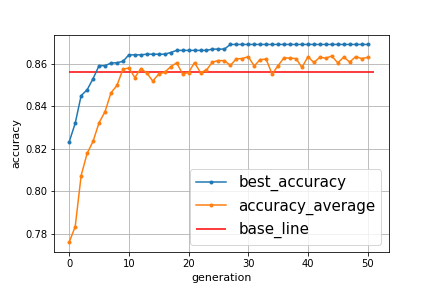
\includegraphics[scale=0.6]{graph.png}
	\caption{accuracyの推移\label{fig:graph1}}
\end{figure}
最終的な最良値は0.8691となった.\\
適用確率を追加前の最良値は0.8676であり,
あまり改善があったとはいえない.

\section{実験2}
実験1で得られた個体を用いてアンサンブル学習を行うことで精度を高めることを試みた.

\subsection{実験2.1}
表\ref{tb:param2}に学習パラメータを示す.

\begin{table}[h]
	\centering
	\caption{学習パラメータ\label{tb:param2}}
	\scalebox{1.0}{
		\begin{tabular}{|c||c|} \hline
			optimizer&Adam\\ \hline
			learning rate&0.001\\ \hline
			loss function&categorical\_crossentropy\\ \hline
			batch size&128\\ \hline
			epoch&100\\ \hline
		\end{tabular}
	}
\end{table}
元のデータ数は50000とした.
まず,上位3個体を用いて,2倍に水増して学習させ,予測したものの平均をとり,最終的な予測値とした.
また,対照実験は上位3個体のいずれかを適用する操作で6倍に水増しして学習,予測を行った.
表\ref{tb:res1}に実験結果を示す.\\
\begin{table}[h]
	\centering
	\caption{実験結果\label{tb:res1}}
	\scalebox{1.0}{
		\begin{tabular}{|c||c|} \hline
			1st&0.9044\\ \hline
			2nd&0.9006\\ \hline
			3rd&0.9037\\ \hline
			ensemble&0.9141\\ \hline
			control&0.8963\\
			experiment&\\ \hline
		\end{tabular}
	}
\end{table}
アンサンブル学習は他のものとくらべ1\%ほどの改善が見られ,アンサンブル学習の効果が表れていることが分かる.\\ \\

次に表\ref{tb:res2}に上位10個体を用いてアンサンブル学習を行った結果を示す.
ただし,10個体のうちどの個体を用いるかを全探索によって調べ上げ最良のものとした.
また,各個体の学習についてのaccuracyについて最良のものではなく最終のもので行った.
\begin{table}[h]
	\centering
	\caption{実験結果\label{tb:res2}}
	\scalebox{1.0}{
		\begin{tabular}{|c||c|} \hline
			\rowcolor[rgb]{0,0.9,0.9}
			1st&0.9044\\ \hline
			\rowcolor[rgb]{0,0.9,0.9}
			2nd&0.9006\\ \hline
			\rowcolor[rgb]{0,0.9,0.9}
			3rd&0.9037\\ \hline
			4th&0.8386\\ \hline
			\rowcolor[rgb]{0,0.9,0.9}
			5th&0.8541\\ \hline
			\rowcolor[rgb]{0,0.9,0.9}
			6th&0.8624\\ \hline
			7th&0.8608\\ \hline
			8th&0.8565\\ \hline
			9th&0.8740\\ \hline
			\rowcolor[rgb]{0,0.9,0.9}
			10th&0.8596\\ \hline
			ensemble&0.9205\\ \hline
		\end{tabular}
	}
\end{table}
色を付けたものがアンサンブルに使われた個体である.
このことから上位個体だけよりもさらに複数の個体を組み合わせることで多少の改善が行われることが分かる.
また,上位3個体についてGAで非常に良い個体が選ばれていたことがい伺える.
一方でそれ以外の個体は順位通りとはいかないようなaccuracyとなっており,これは個体の学習時に
学習データをランダムにとってきているのでそれに合わせた個体になっていると考えられる.
このことから,個体の適応度を算出するのにデータ数を多くする,
あるいは複数回の学習の平均をとらなければならないことが考えられる.\\ \\ 

\subsection{実験2.2}
さらに表\ref{tb:res3}に上位20個体を用いてアンサンブル学習を行った結果を示す.
ただし,20個体のうちどの個体を用いるかを全探索によって調べ上げ最良のものを示す.
また,今回は元データ5000枚を2倍に水増しして行った.
色を付けたものがアンサンブルに使われた個体である.
\begin{table}[h]
	\centering
	\caption{実験結果\label{tb:res3}}
	\scalebox{1.0}{
		\cellcolor[rgb]{0,0.9,0.9}
		\begin{tabular}{|c|c||c|c|} \hline
			1st&0.7982&
			\cellcolor[rgb]{0,0.9,0.9}2nd&\cellcolor[rgb]{0,0.9,0.9}0.8149\\ \hline
			3rd&0.8055&
			\cellcolor[rgb]{0,0.9,0.9}4th&\cellcolor[rgb]{0,0.9,0.9}0.8107\\ \hline
			5th&0.8075&
			6th&0.8048\\ \hline
			7th&0.7997&
			8th&0.8123\\ \hline
			\cellcolor[rgb]{0,0.9,0.9}9th&\cellcolor[rgb]{0,0.9,0.9}0.8101&
			10th&0.8064\\ \hline
			\cellcolor[rgb]{0,0.9,0.9}11st&\cellcolor[rgb]{0,0.9,0.9}0.8041&
			12nd&0.7966\\ \hline
			\cellcolor[rgb]{0,0.9,0.9}13rd&\cellcolor[rgb]{0,0.9,0.9}0.8091&
			14th&0.8087\\ \hline
			15th&0.7980&
			16th&0.8066\\ \hline
			\cellcolor[rgb]{0,0.9,0.9}17th&\cellcolor[rgb]{0,0.9,0.9}0.8072&
			\cellcolor[rgb]{0,0.9,0.9}18th&\cellcolor[rgb]{0,0.9,0.9}0.8094\\ \hline
			19th&0.7977&
			20th&0.8028\\ \hline
			\multicolumn{2}{|c|}{ensemble}&\multicolumn{2}{|c|}{0.8568}\\ \hline
		\end{tabular}
	}
\end{table}

アンサンブル学習の効果自体は非常によく見て取れるが,バグったのかaccuracyが全体を通して小くなってしまった.

\section{今後の課題}
\begin{itemize}
	\item 適応度の計算の際に複数回学習を行うのかデータ数を増やしたほうがいいのか
	\item アンサンブル学習を最終的に行うことを前提とした個体選択ができないのか
\end{itemize}

\end{document}


